\chapter{Clases}
\section{Introduccion}
\begin{center}
Introduccion
\end{center}

\begin{flushleft}
Los diagramas de clases son diagramas estructurales del lenguaje unificado de modelado o UML (unified modeling language). Este lenguaje de modelado visual es un estándar ISO para visualizar los sistemas de la programación orientada a objetos, aunque también permite visualizar procesos de negocio. Con ayuda de elementos gráficos, UML muestra los estados de los sistemas y describe las interacciones entre los elementos que lo componen.
\\ 
Los diagramas de clases son diagramas estructurales del lenguaje unificado de modelado o UML (unified modeling language). Este lenguaje de modelado visual es un estándar ISO para visualizar los sistemas de la programación orientada a objetos, aunque también permite visualizar procesos de negocio. Con ayuda de elementos gráficos, UML muestra los estados de los sistemas y describe las interacciones entre los elementos que lo componen.
\end{flushleft}
\newpage
\section{Descripción}
\begin{flushleft}En esta oportunidad diseñamos un diagrama de clase para nuestro proyecto utlizando la herramienta Coloso, donde diseñamos una estructura de lo que seria nuestro proyecto,	se crearon las entidades base de cliente y gestor, que heredan de una clase Usuario, al igual se creo una entidad Parqueadero, con ciertos atributos y operaciones.
	\\Se implementaron tres patrones de diseño Gof, que son, Strategy, Command, y Factory Method, el strategy esta pensado para calcular una tarifa designada al parqueo, dependiendo del tipo de vehiculo que se vaya a estacionar, donde el algoritmo base es "calcularTarifa", el patron Factory Method esta pensado para la creacion de los distintos espacios diferenciados por el tipo de vehiculo que van a alojar, por lo tanto, se crea una factoria de espacio de parqueo, y de ella heredan los distintos tipos de espacios que se van a crear, ya que cada uno tiene unas caracteristicas distintas, y por ultimo se penso en el patron command como una forma de verificar si un espacio de parqueo se encuentra actualmente disponible, o , ocupado, y ya terminando con el diseño se agrego una entidad interface que tiene una operacion que activa o muestra la posicion en un mapa de geolocalizacion (con una API de google) correspondiente a la busqueda del usuario. \end{flushleft}

\newpage
\section{Diagrama de Clase UML}
\begin{flushleft}
Para este diagrama se separaron cuatro frames en particular para una mejor interpretacion, los tres frames mas grandes representan los tres patrones de diseño que se planean utilizar en el proyecto, y que van a ser explicados en la siguiente seccion, y un cuarto frame que representa la GUI del proyecto, que va a contar con una interfaz grafica principal del presente proyecto.
\end{flushleft}

{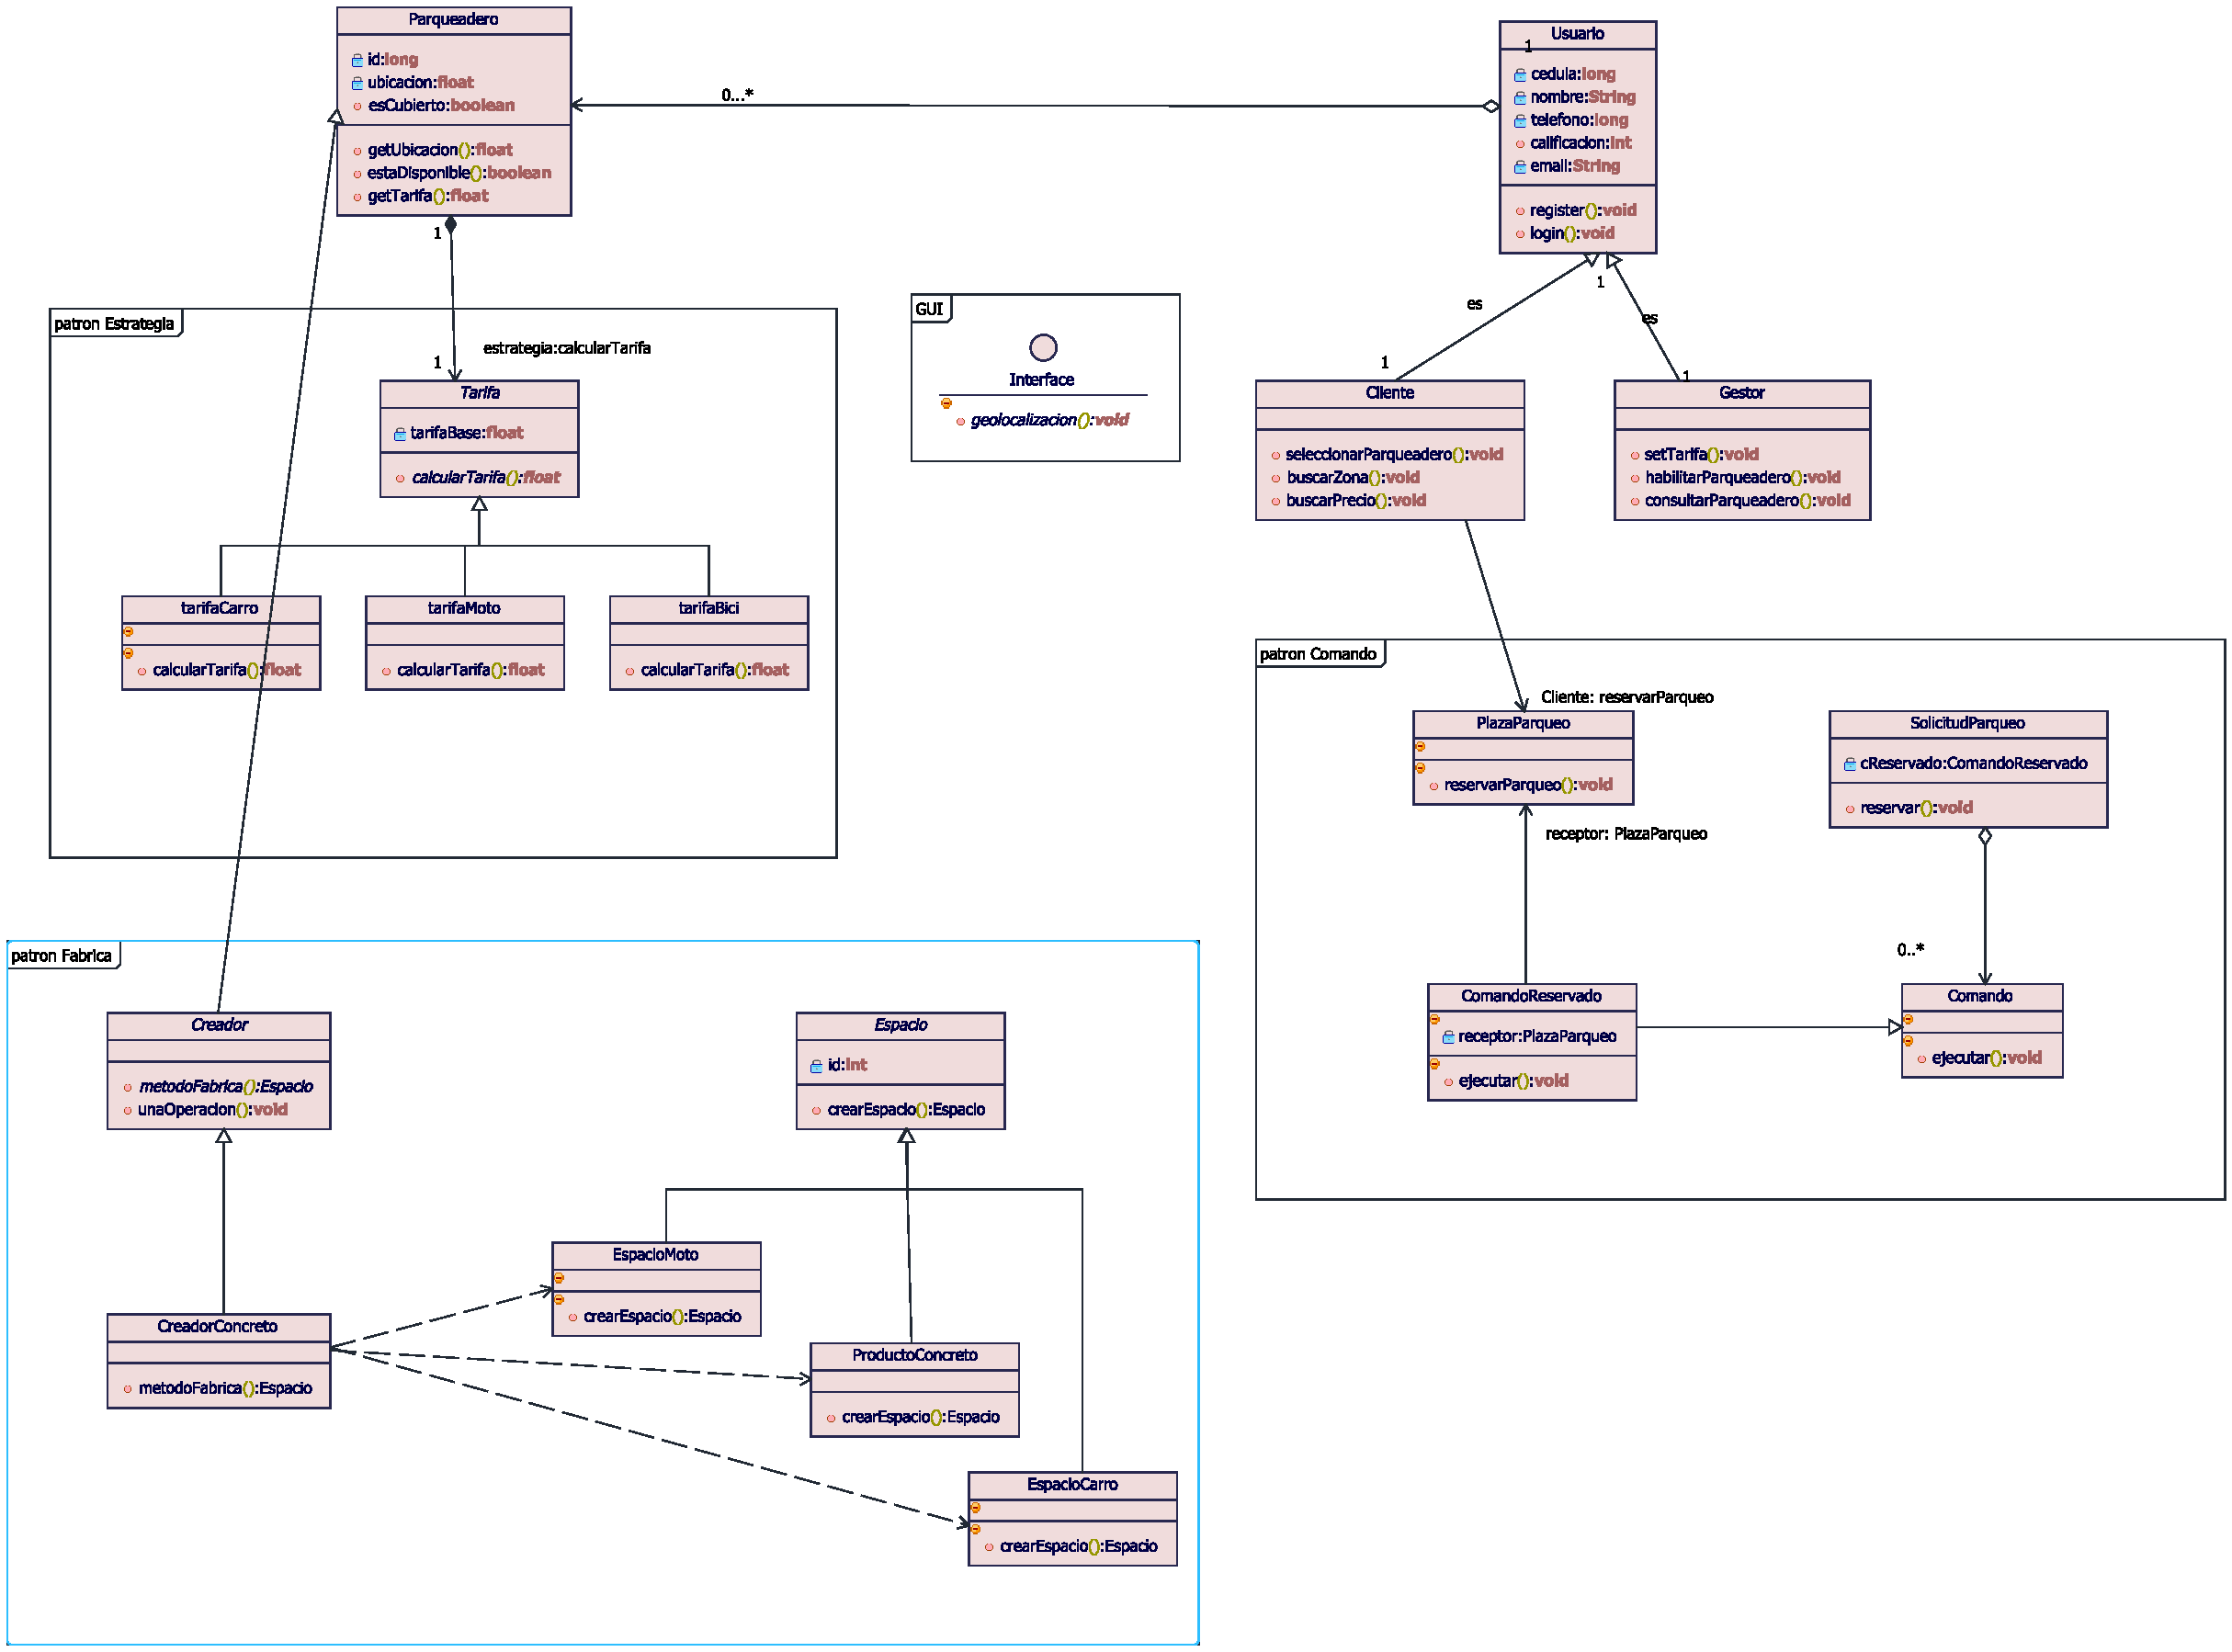
\includegraphics[width=1.38\linewidth]{imgs/DiagramaClase/DiagramaClase}}
\newpage
\section{Diagrama de Clase UML: Patrones de Diseño}
\subsection{Patrón: Estrategia}
\begin{flushleft}
    Este patrón define un conjunto de algoritmos, encapsula cada uno de ellos y los hace intercambiables. Permite que el algoritmo pueda variar independientemente de los clientes que lo utilicen.

Esto quiere decir que nuestros objetos deben estar preparados para afrontar diversos contextos sin cambiar las interacciones de estos con el cliente.

Para este caso concreto, nuestro contexto base va a ser la entidad parqueadero, y nuestro algoritmo principal es calcularTarifa, asi el cliente, dependiendo el tipo de parqueo que seleccione, va a pedir calcular una tarifa determinada para el tipo de vehiculo que halla seleccionado.
\\

\end{flushleft}

\begin{center}
{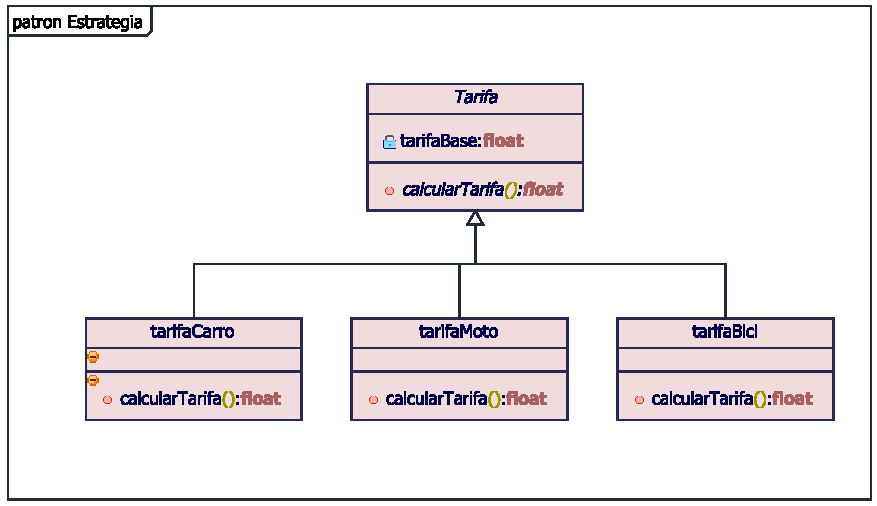
\includegraphics[width=1.15\linewidth]{imgs/DiagramaClase/Strategy}}
\end{center}
\begin{center}
	Figura 0.0. En este caso nuestro contexto va a ser "Parqueadero" (Se puede ver en el diagrama de clases general) y nuestra Interface del Algoritmo va a ser "calcularTarifa", el cual es un algoritmo que varia en funcion del vehiculo que se vaya a estacionar
\end{center}
\newpage

\subsection{Patrón: Método Fábrica}
\begin{flushleft}
	Factory Method permite la creación de objetos de un subtipo determinado a través de una clase Factory. Esto es especialmente útil cuando no sabemos, en tiempo de diseño, el subtipo que vamos a utilizar o cuando queremos delegar la lógica de creación de los objetos a una clase Factory. 
	El patron factory method nos sirve para la creacion de los espacios teniendo en cuenta si el vehiculo es una bicicleta, creara un espacio para una bicicleta, si entra un carro un espacio de carro y asi dependiendo el requerimiento solicitado.
	\\
	
\end{flushleft}

\begin{center}
	{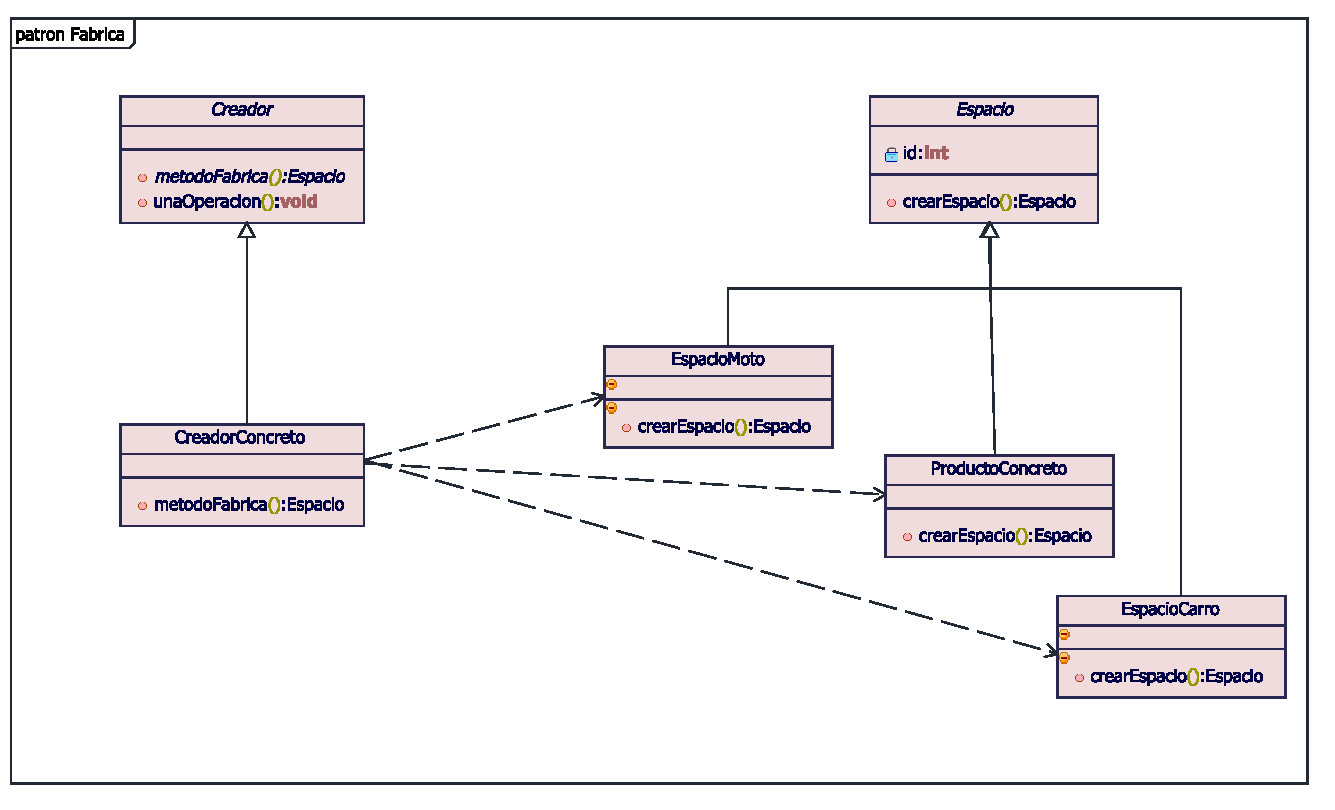
\includegraphics[width=1.20\linewidth]{imgs/DiagramaClase/FactoryMethod}}
\end{center}
\begin{center}
	Figura 0.0. Patron Factory Method para la creacion de distintos espacios de estacionamiento
\end{center}
\newpage

\subsection{Patrón: Comando}
\begin{flushleft}
	El patrón de diseño Command es muy utilizado cuando se requiere hacer ejecuciones de operaciones sin conocer realmente lo que hacen, estas operaciones son conocidas como comandos y son implementadas como una clase independiente que realiza una acción muy concreta, para lo cual,únicamente recibe un conjunto de parámetros para realizar su tarea.
	Se usa el patrón command para recibir las peticiones de los usuarios denominados clientes de manera encapsulada, esto con el objetivo de separar la lógica de la interfaz, en este patrón con el comando reservado se envía la petición de reservar una plaza en el parqueadero previamente seleccionado, esto permitirá controlar las peticiones y decidir si es disponible aparcar o no en el sitio seleccionado.
	\\
	
\end{flushleft}

\begin{center}
	{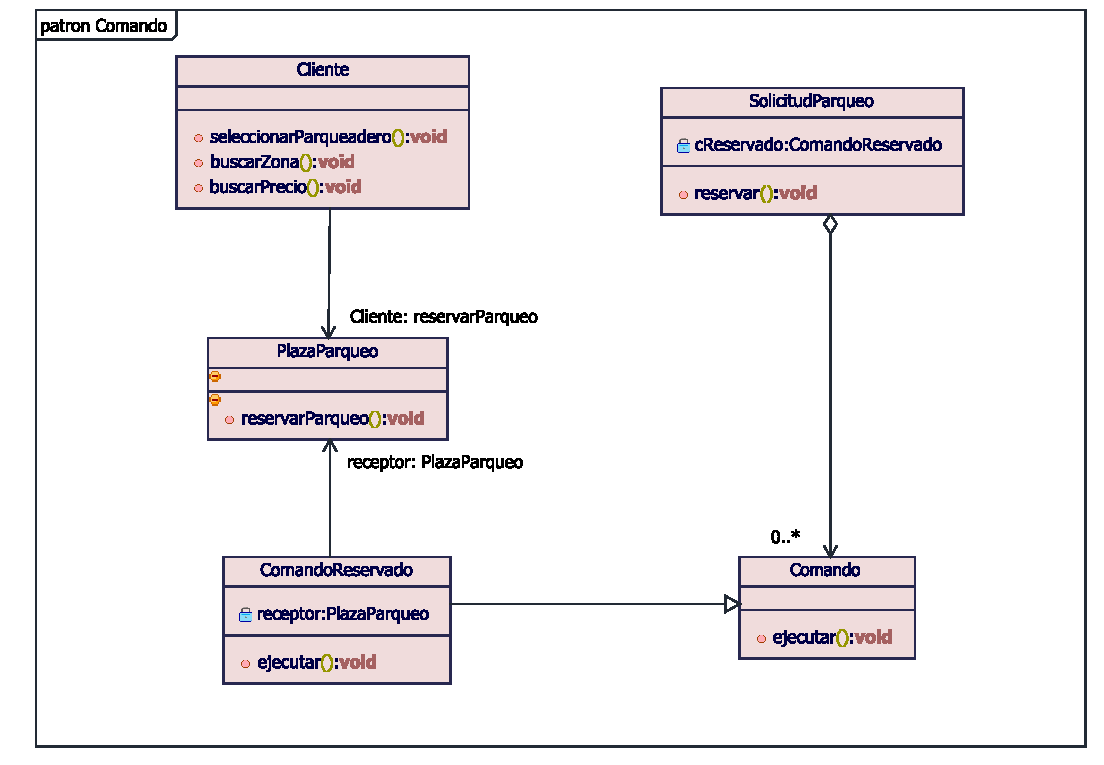
\includegraphics[width=1.20\linewidth]{imgs/DiagramaClase/command}}
\end{center}
\begin{center}
	Figura 0.0. Patron Comando para la validacion de disponibilidad de un espacio de parqueo concreto
\end{center}
\newpage
